\chapter{Design}

\subsection{Concept}
This chapter will explain the design answer for the reports final problem statement. (see \autoref{sec:FPS}) The purpose of this report design chapter is to produce an interactive physical object to answer the final problem statement. 

\subsection{Intial design}
\setlength{\parskip}{1em}

\setlength{\parindent}{10ex}
To create the initial design for the physical interface, the project group started to sketch ideas based on the research gathered from the analysis. The main task was to make ideas based on collaboration which was one of the directions this report concentrates on. The directions were either cooperative, interaction, and collaboration. These directions are what the paper prototypes are made to represent.\par

\setlength{\parindent}{10ex}
The paper prototypes where presented in a classroom at Sankt Annæ. Each 6 members of the group presented their idea for a group between 4-6 children and received feedback for further understanding of the target group. It was found out that the target group wanted more movement, variation, games, visuality, physical and group work. 
The ideas presented at the workshop can be seen in appendix ….XXXX.
The idea behind splitting into individual groups and getting feedback was to gather more diverse sketches. This made it better to gather more information from a various aspect of ideas. The reason for using this approach is to avoid biases from within the group. \par

\setlength{\parindent}{10ex}
After gathering the ideas from the workshop, the whole group divided again to make a new paper prototype to present to each other. This time with focus on the data gathered from the workshop. 
The ideas presented to each other can be seen in appendix ….XXXX. 
Each idea had a prompted outcome from the workshop, but the group wanted to make a design and implementation that involved as many aspects from the workshop as possible. \par

\setlength{\parindent}{10ex}
A list of different pointers was made to make an overview of some of the component and software implementation that is necessary. 
The list of component/software implementation can be seen in appendix ….XXXX. 
The group split up into two groups of 3 people. Using these pointers to make a final idea. 
The two ideas from each group can be seen in appendix …..XXXX. 
The two ideas were then discussed and talked through to finalize the final design. 

\subsection{Final design}
Below is the design concept sketches of the final design. 

\begin{figure}[H]
	\centering
	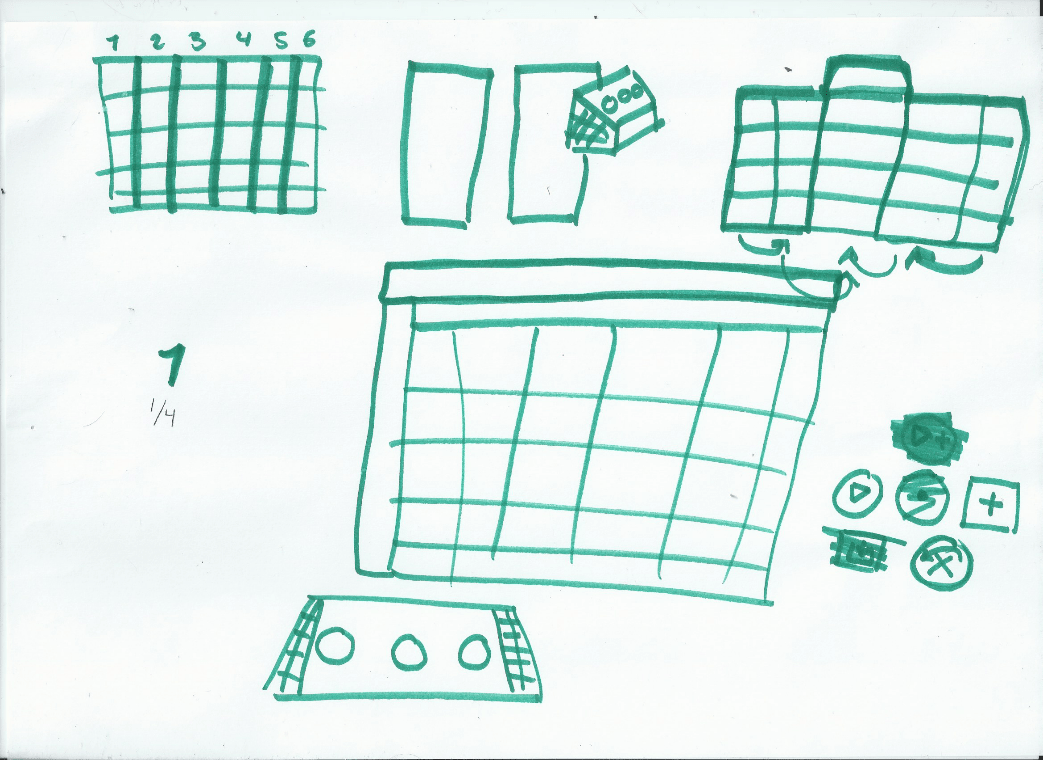
\includegraphics[width=0.7\linewidth]{figure/Design/sketchOne}
	\label{fig:sketchOne}
	\caption{Shows the early stage of the final design}
	
\end{figure}

\begin{figure}[H]
	\centering
	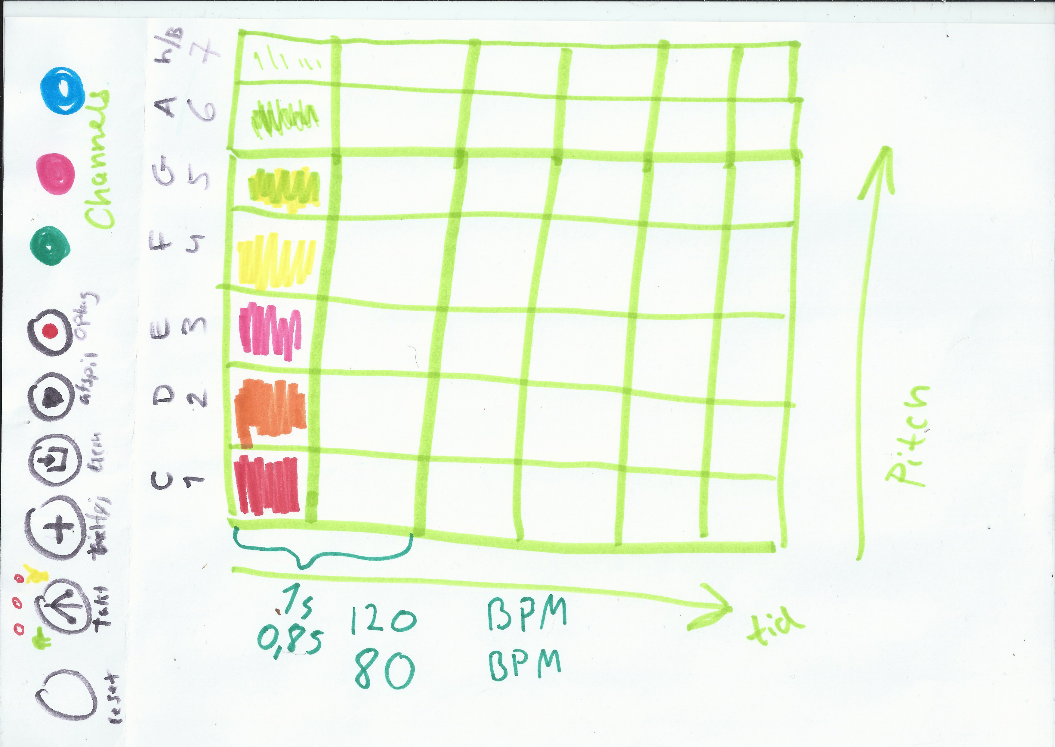
\includegraphics[width=0.7\linewidth]{figure/Design/sketchTwo}
	\label{fig:sketchTwo}
	\caption{Shows the the more completed final design}
	
\end{figure}

\begin{figure}[H]
	\centering
	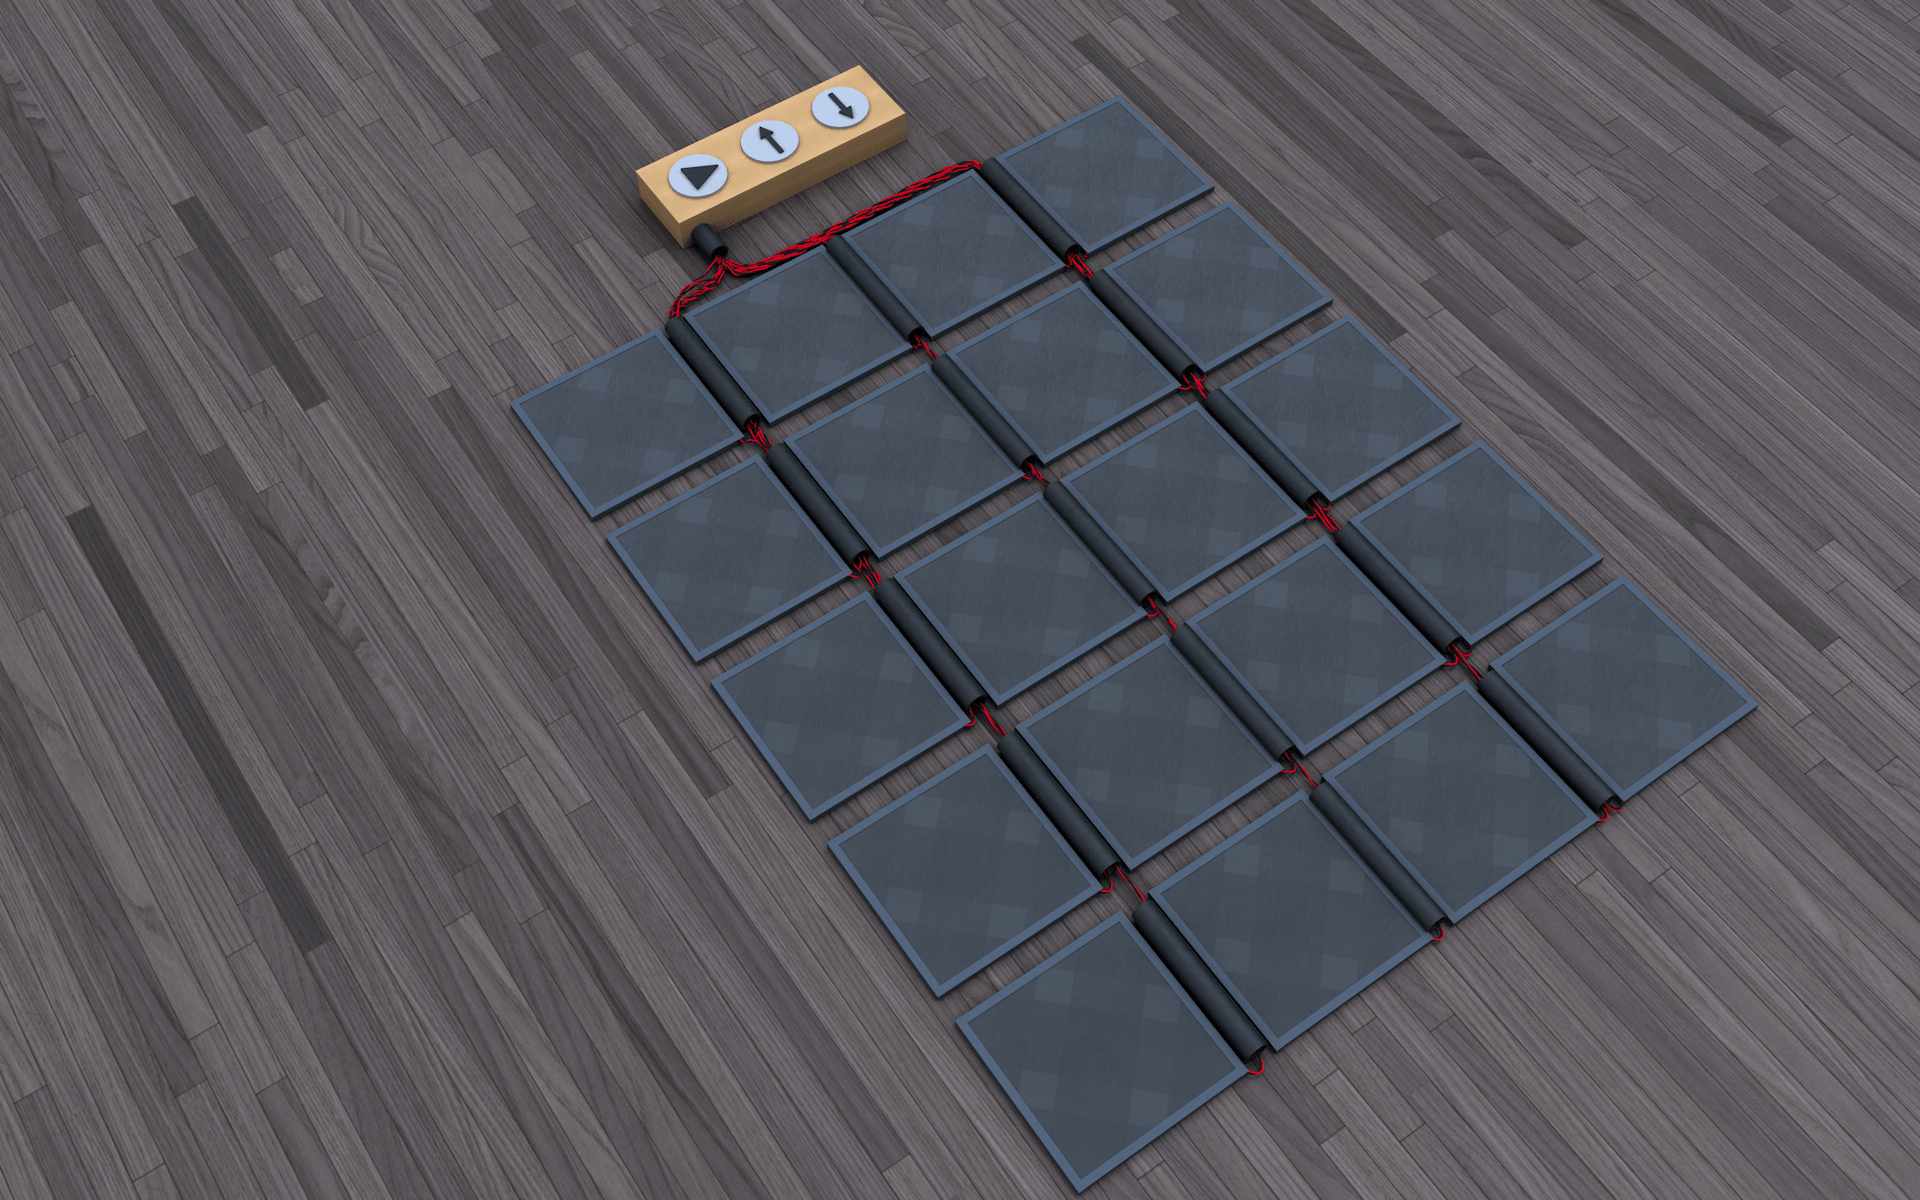
\includegraphics[width=0.7\linewidth]{figure/Design/finaldesign}
	\label{fig:finaldesign}
	\caption{The picture of how the final design should look like}
	
\end{figure}


\subsection{Physical interface}

\subsubsection{Making of the buttons}

The process of the buttons used for the interaction with the mat.

\begin{figure}[H]
	\centering
	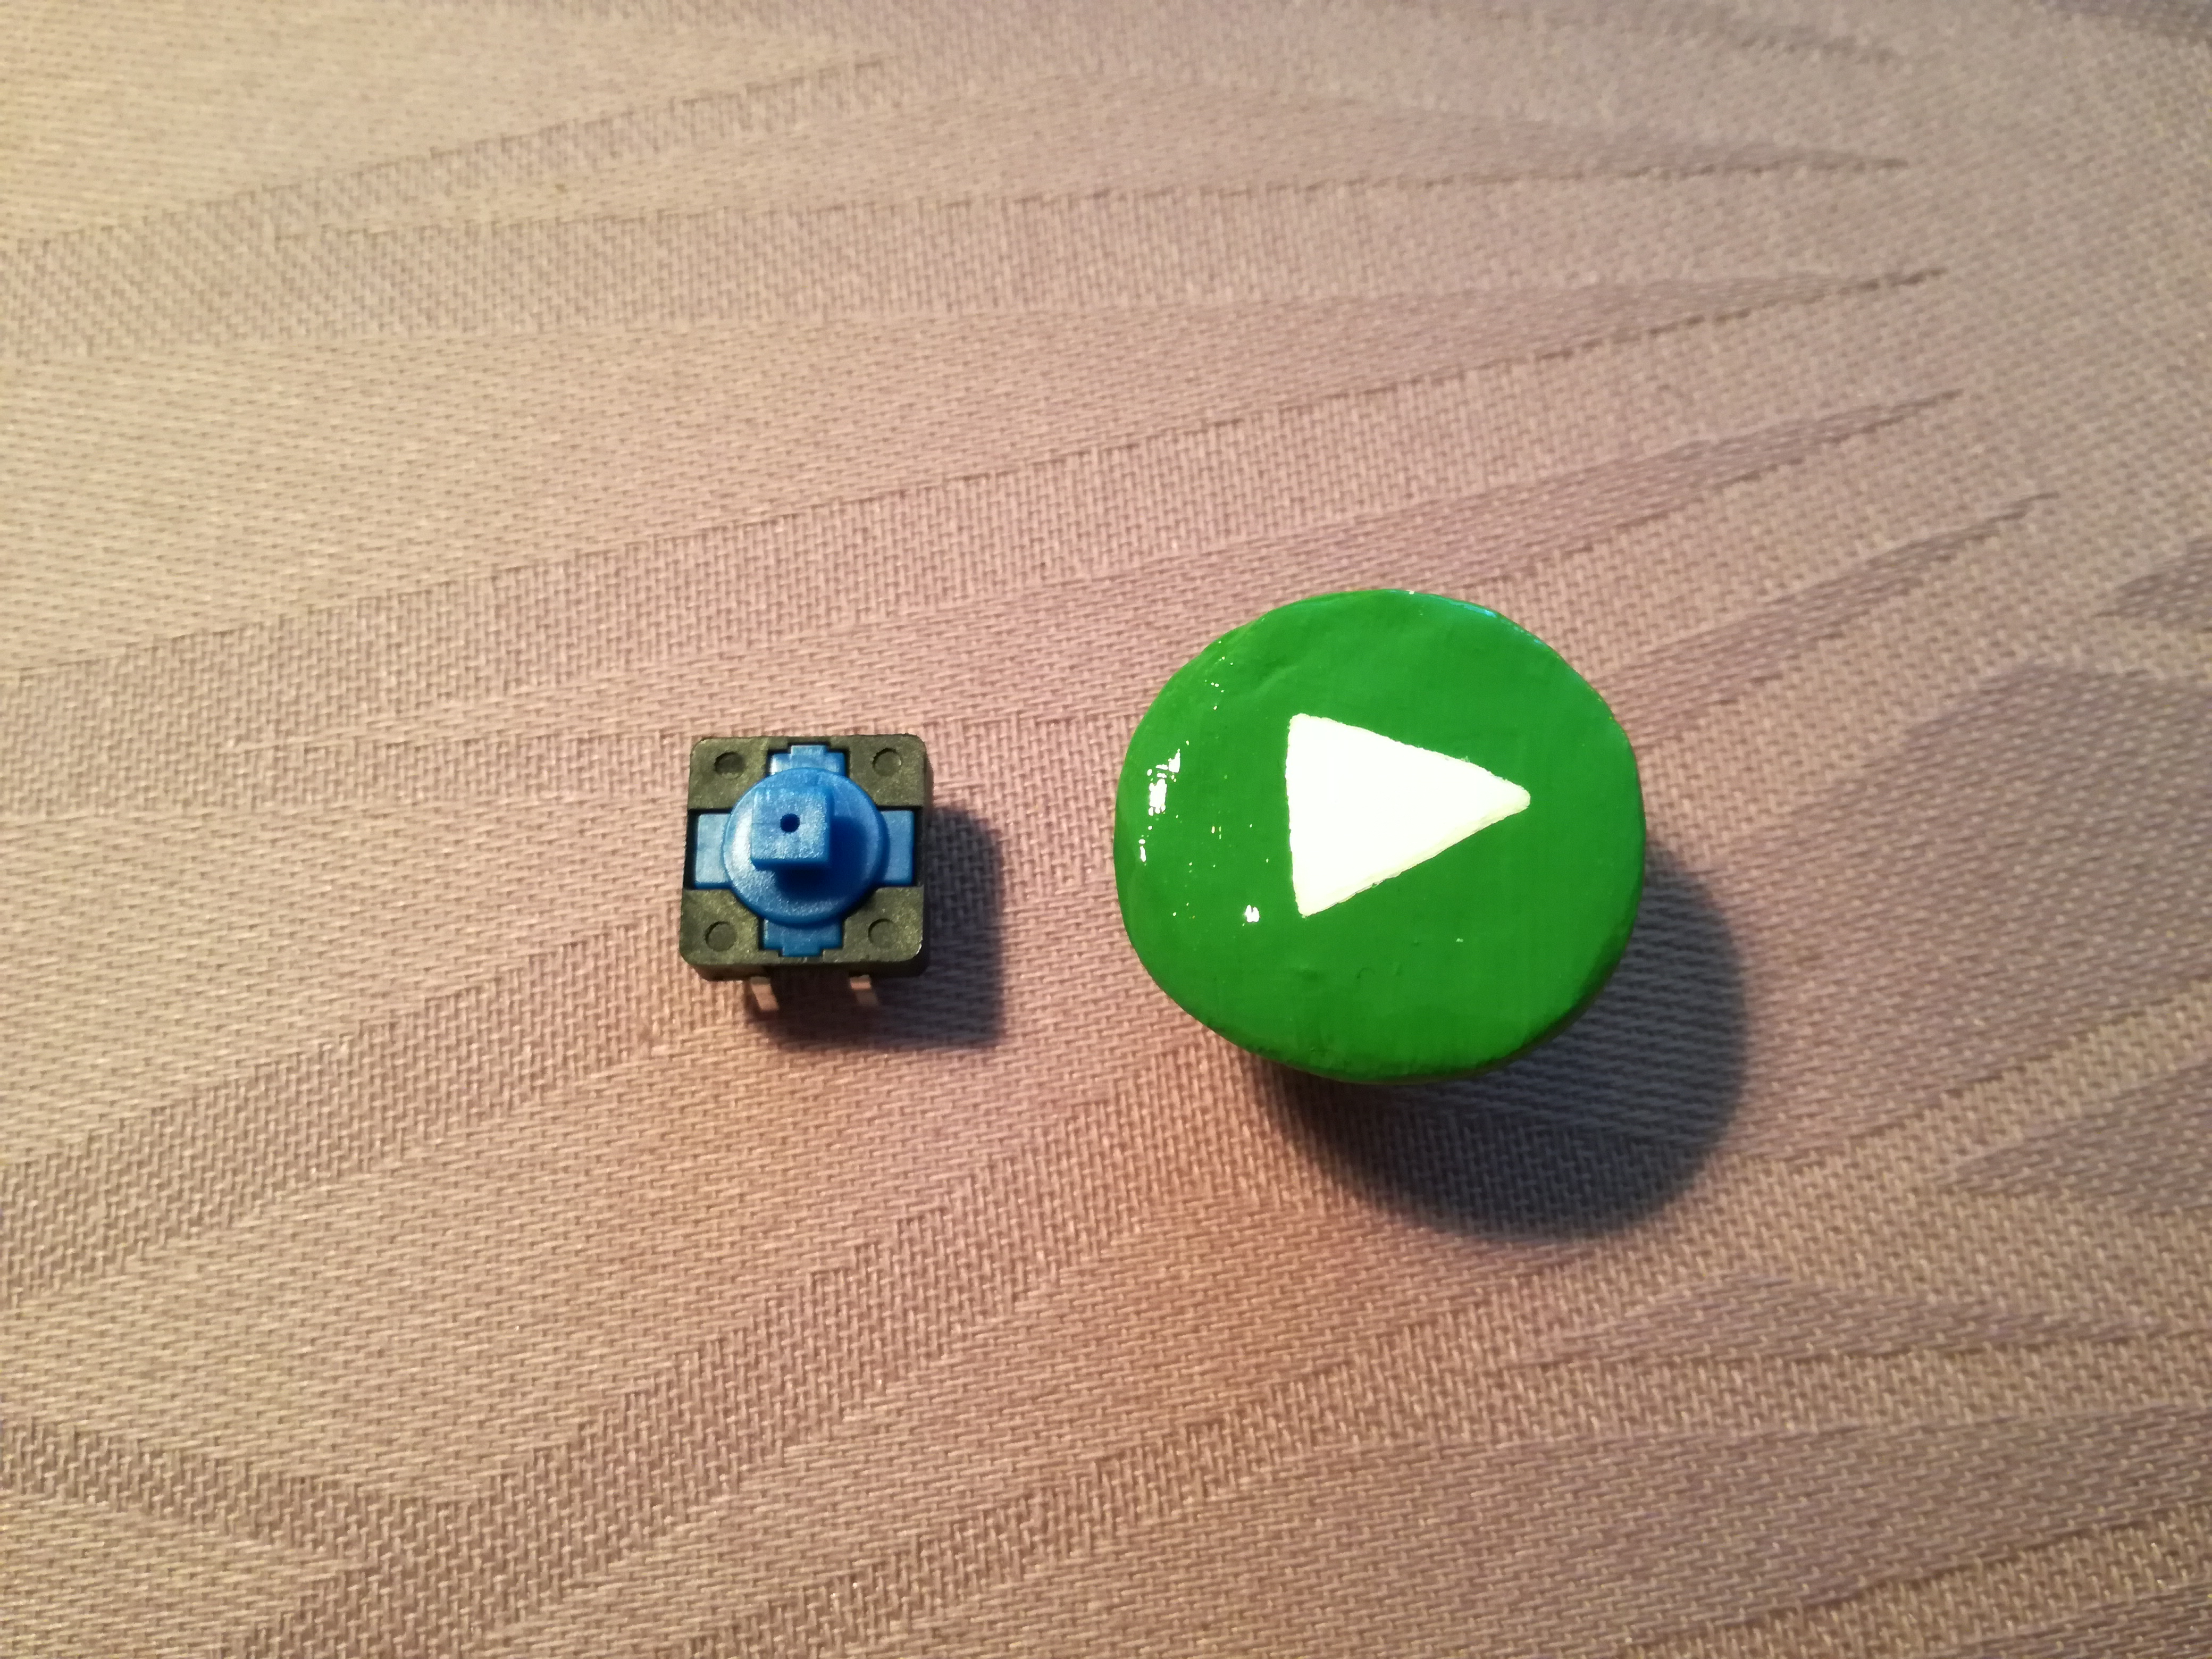
\includegraphics[width=0.7\linewidth]{figure/Design/buttons}
	\label{fig:buttons}
	\caption{On the left is the button without the customized button and on the right is the customized version of the final play button.}
	
\end{figure}

\begin{figure}[H]
	\centering
	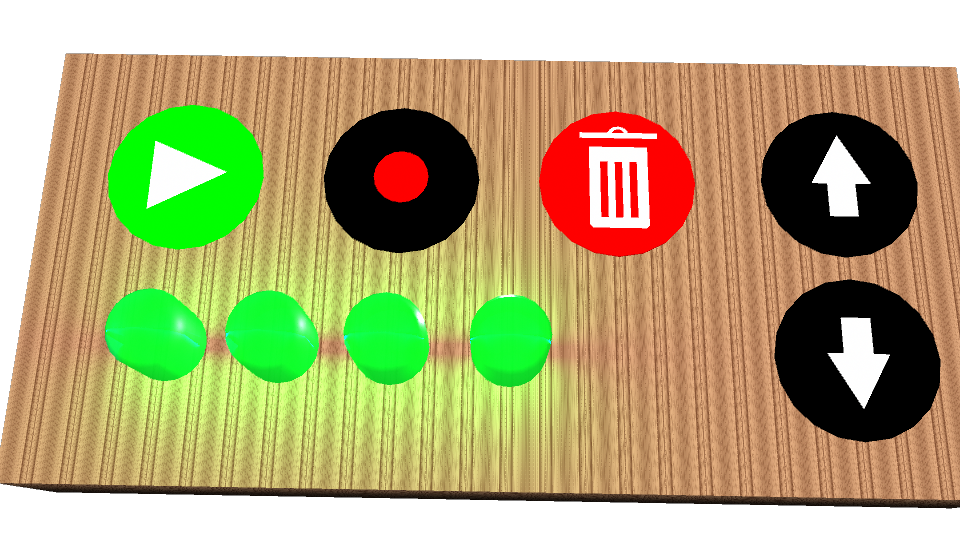
\includegraphics[width=0.7\linewidth]{figure/Design/buttonDesign}
	\label{fig:buttonDesign}
	\caption{The final design on how the buttons should look like and implemented on the prototype.}
	
\end{figure}


\subsubsection{Makings of the mat}

\begin{figure}[H]
	\centering
	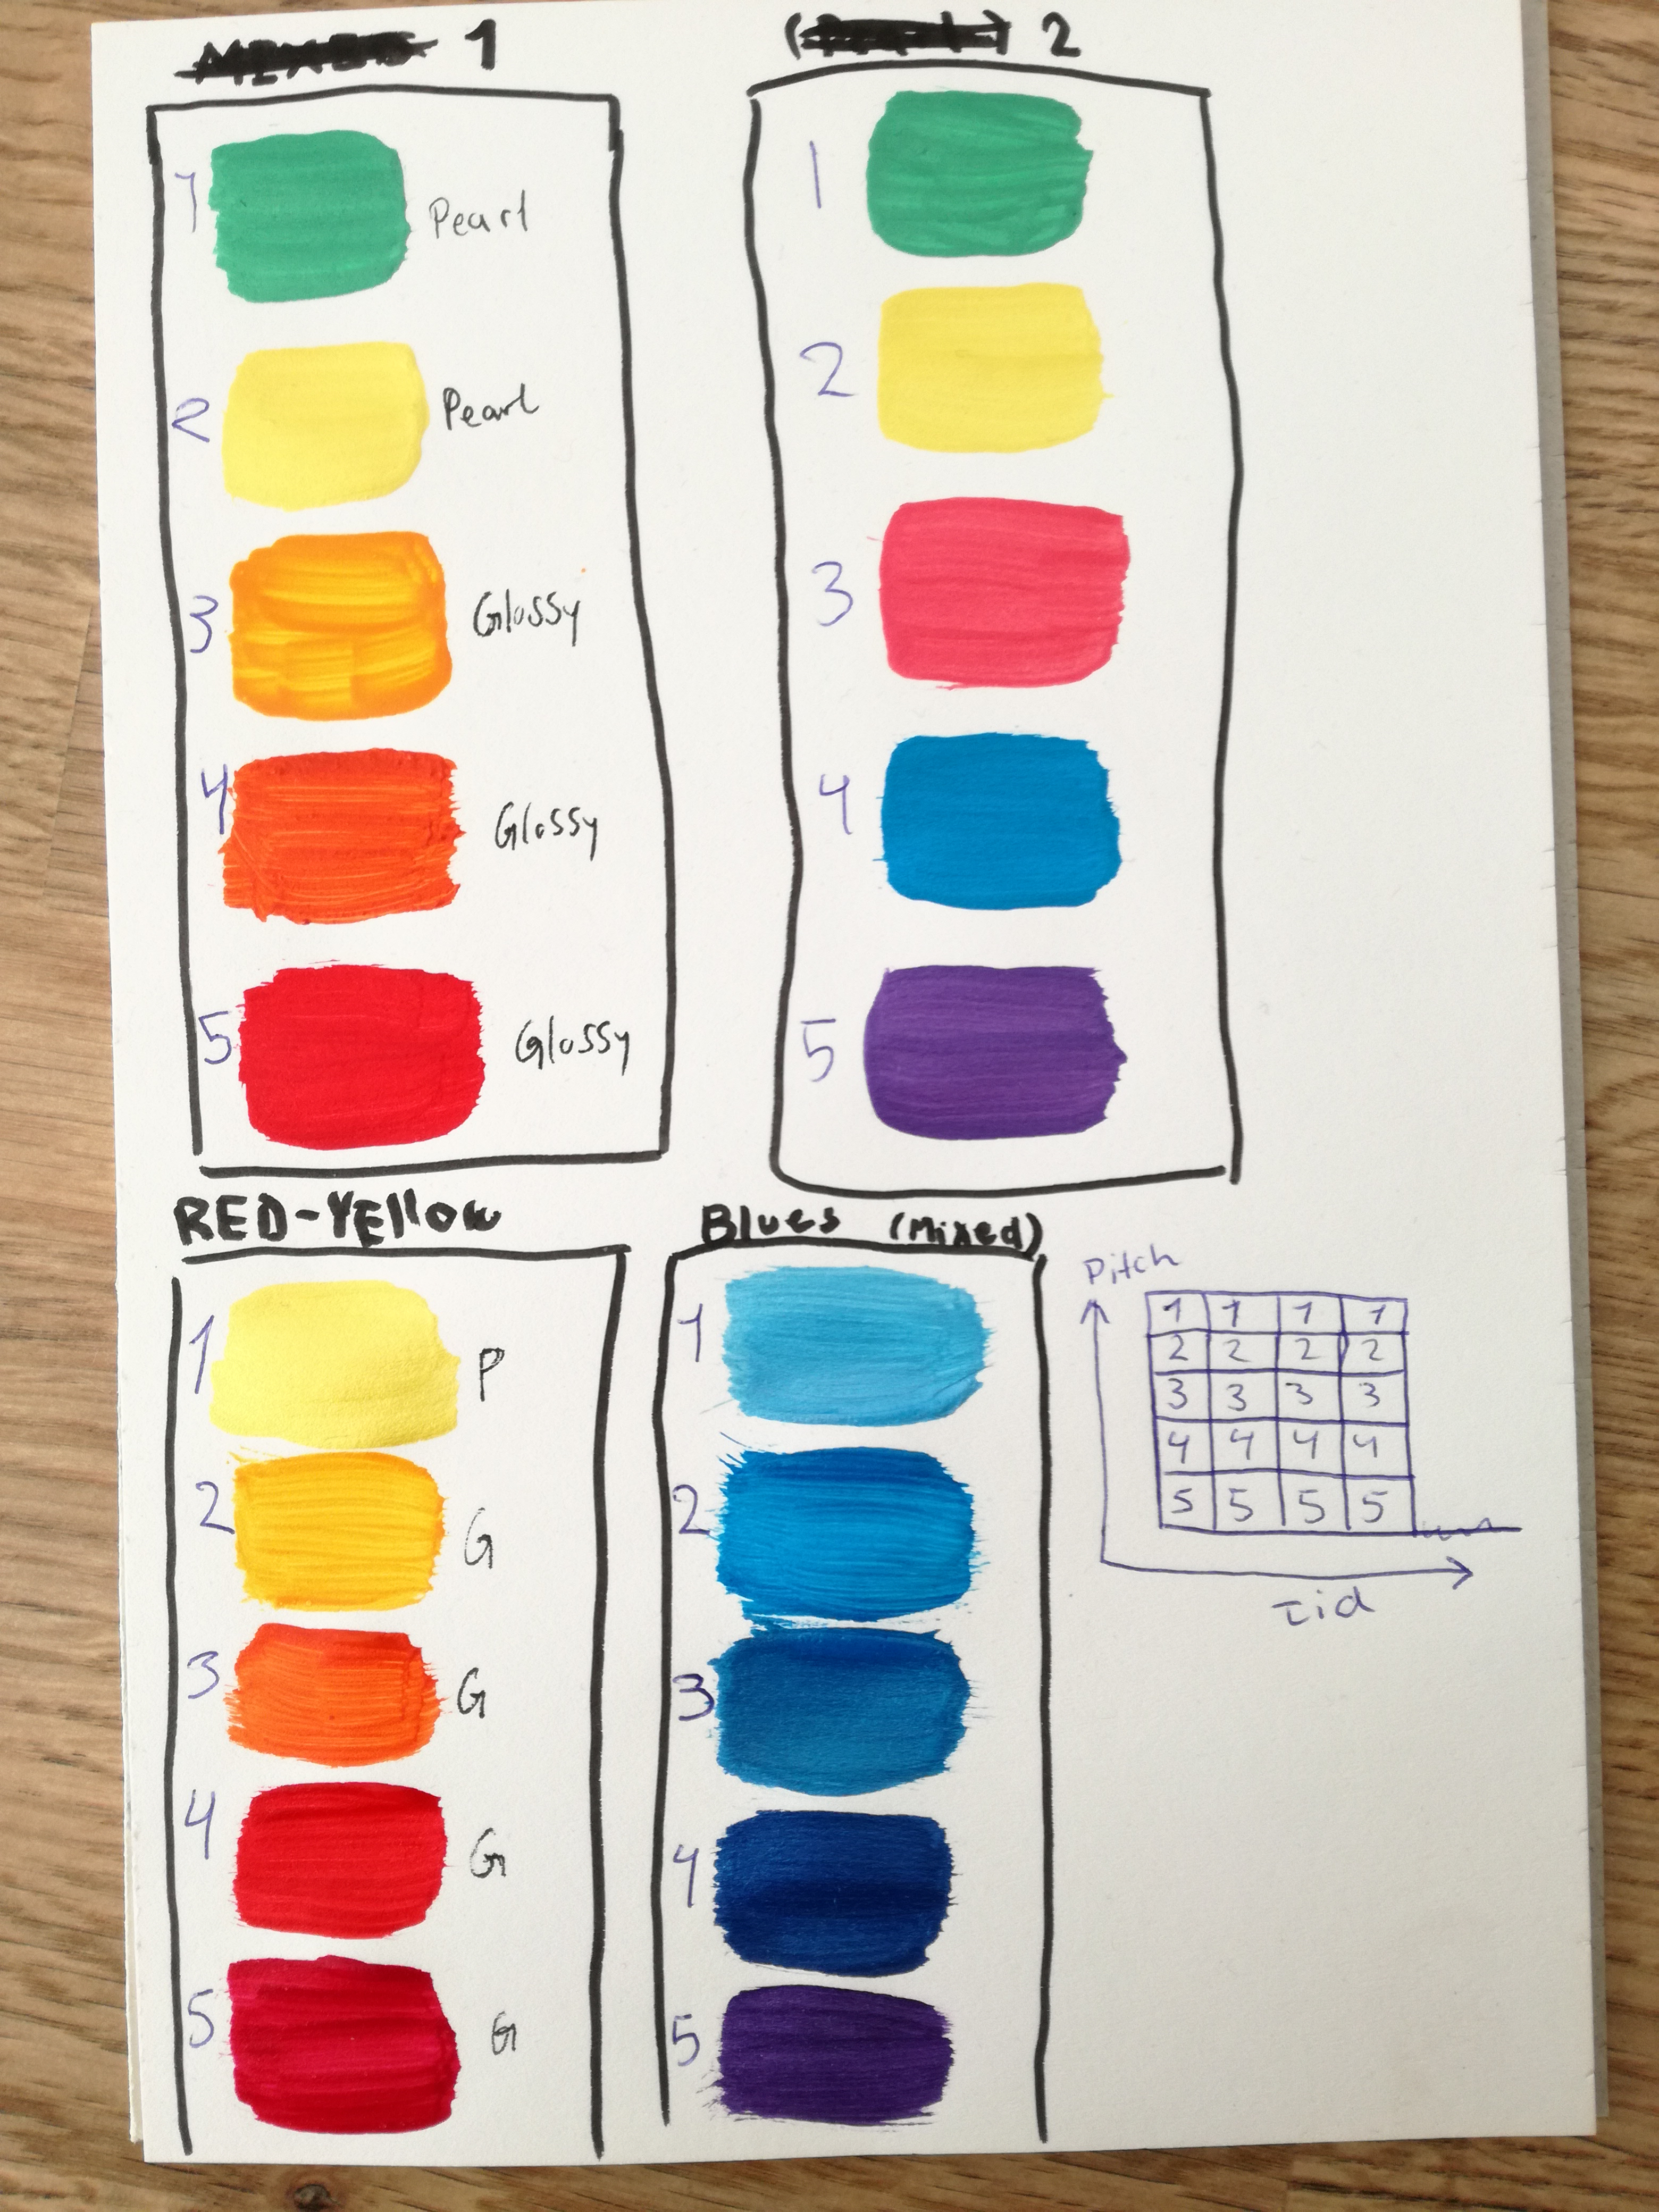
\includegraphics[width=0.7\linewidth]{figure/Design/colors}
	\label{fig:colors}
	\caption{The different color combinations for the mat}
	
\end{figure}

\subsection{The calculations}

\subsection{The result}


\begin{figure}[H]
	\centering
	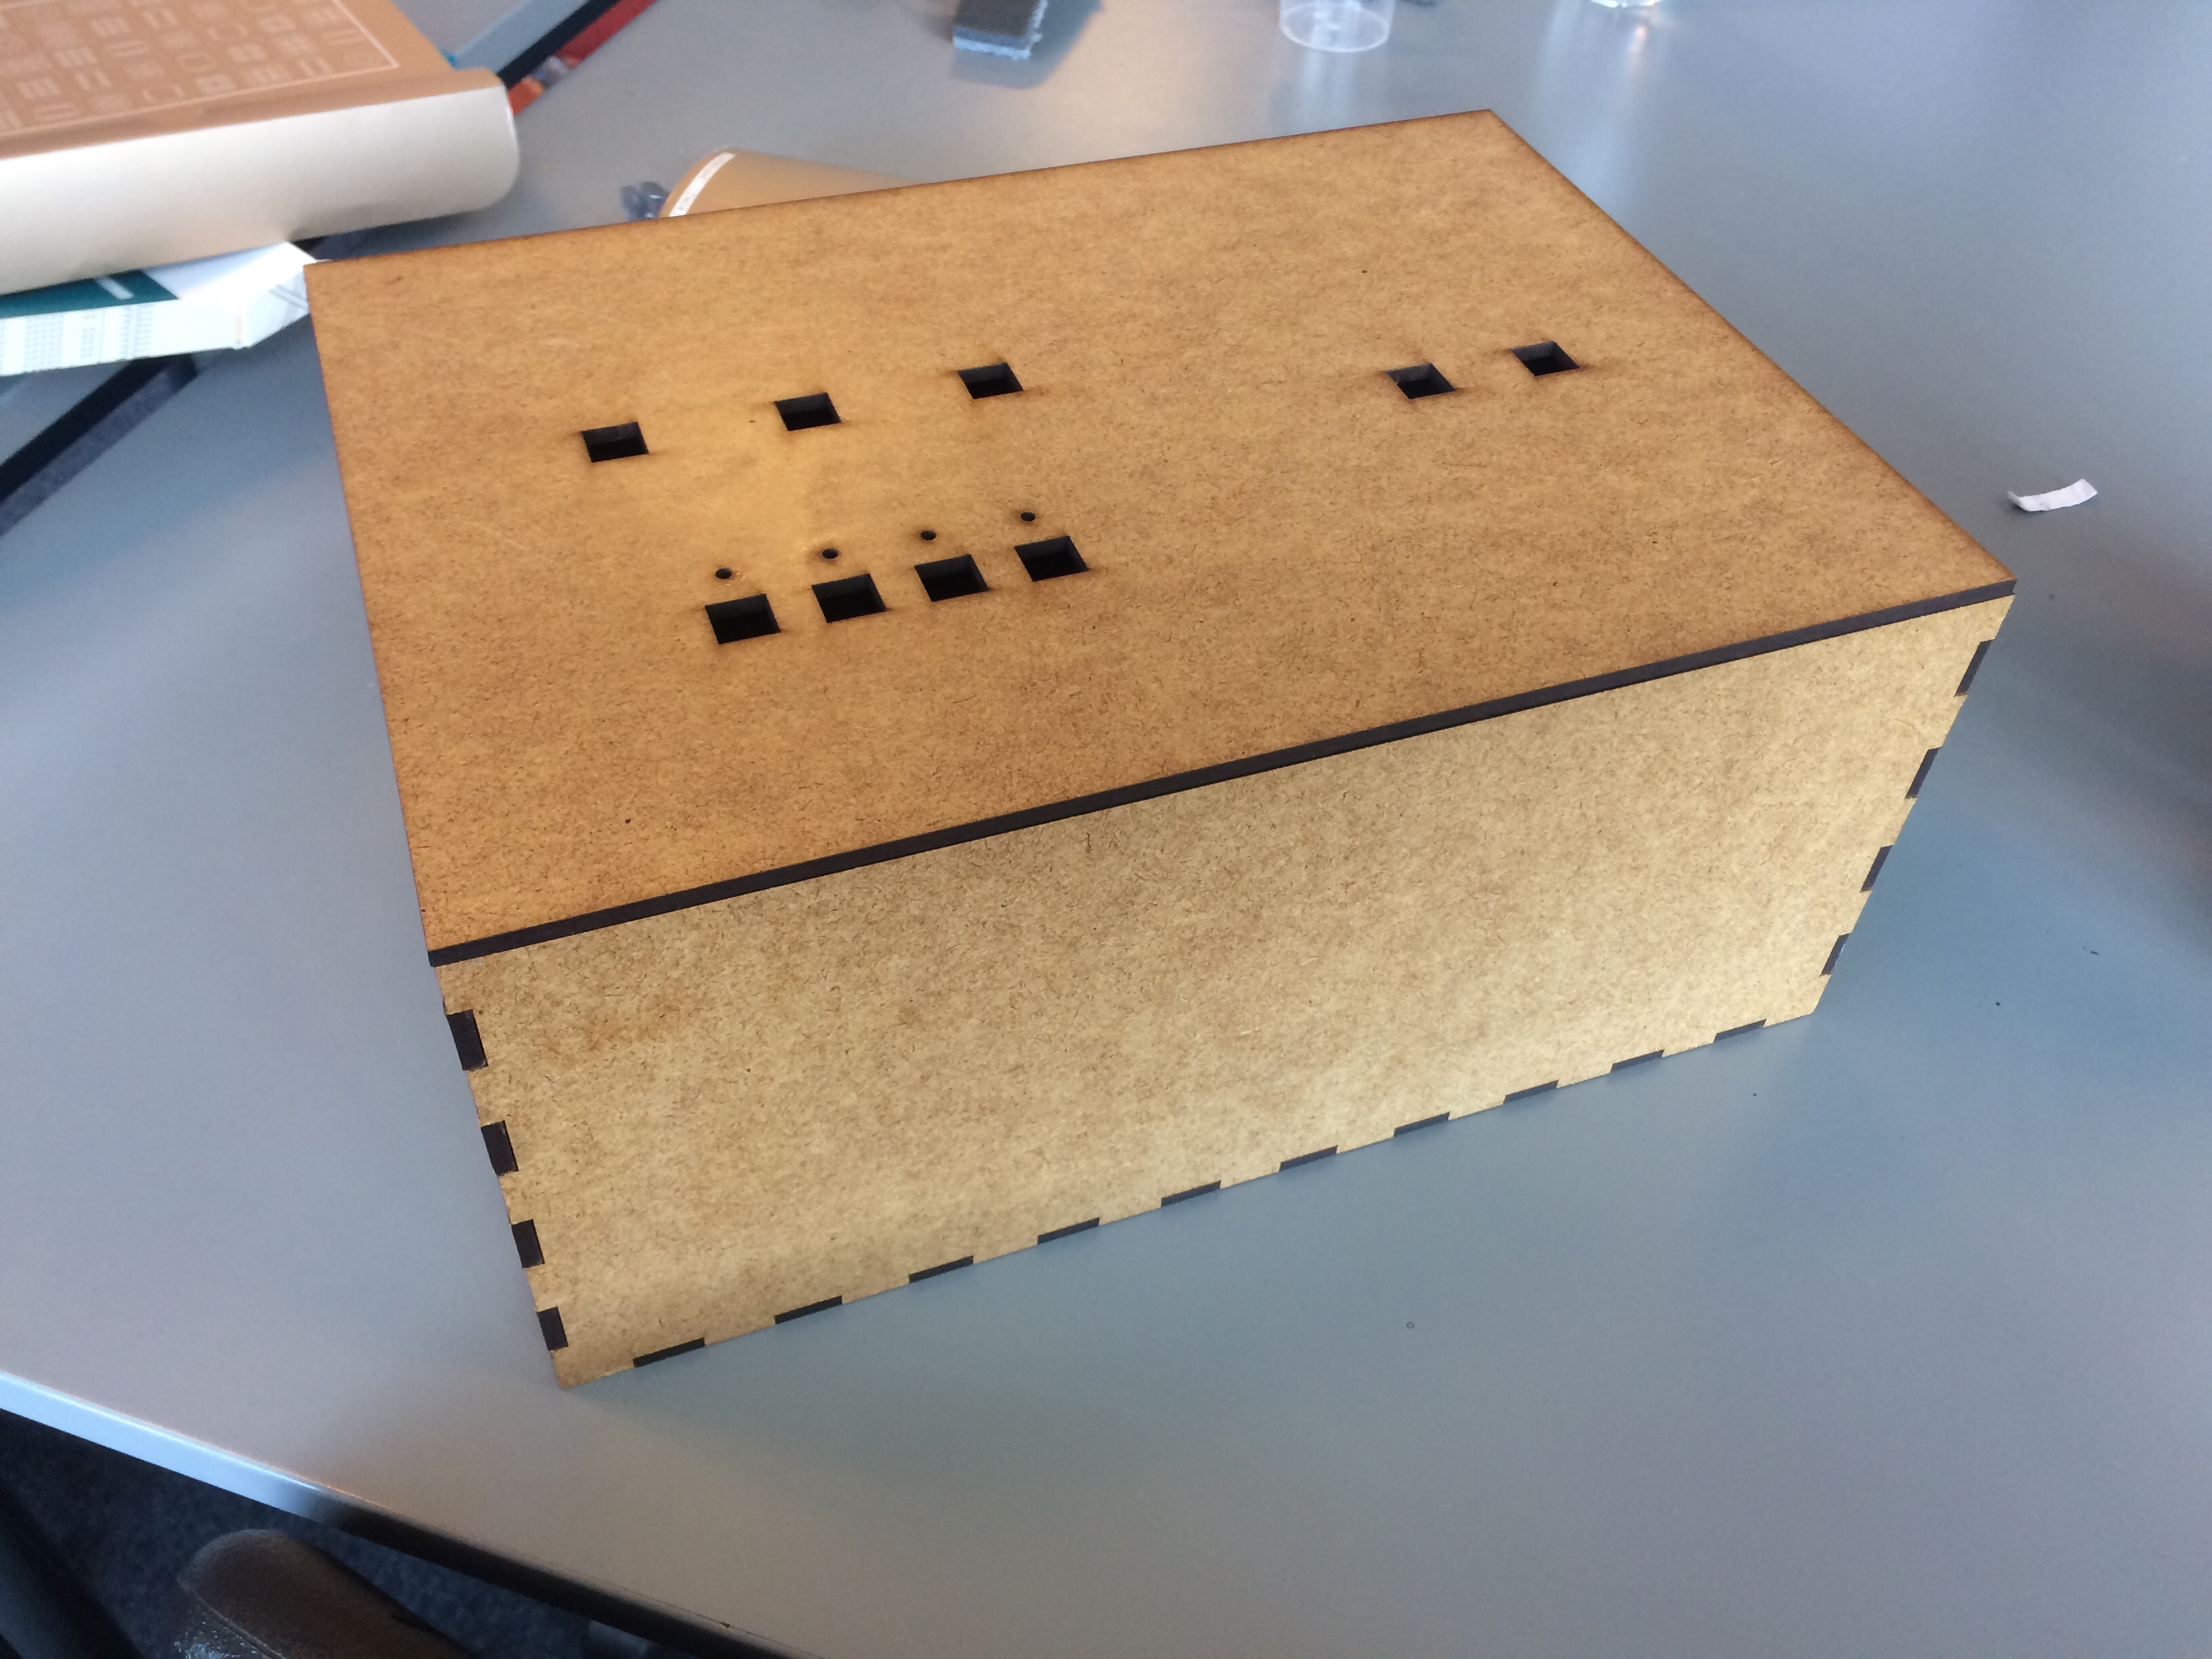
\includegraphics[width=0.7\linewidth]{figure/Design/finalbox1}
	\label{fig:finalbox1}
	\caption{The final prototype box}
	
\end{figure}

\begin{figure}[H]
	\centering
	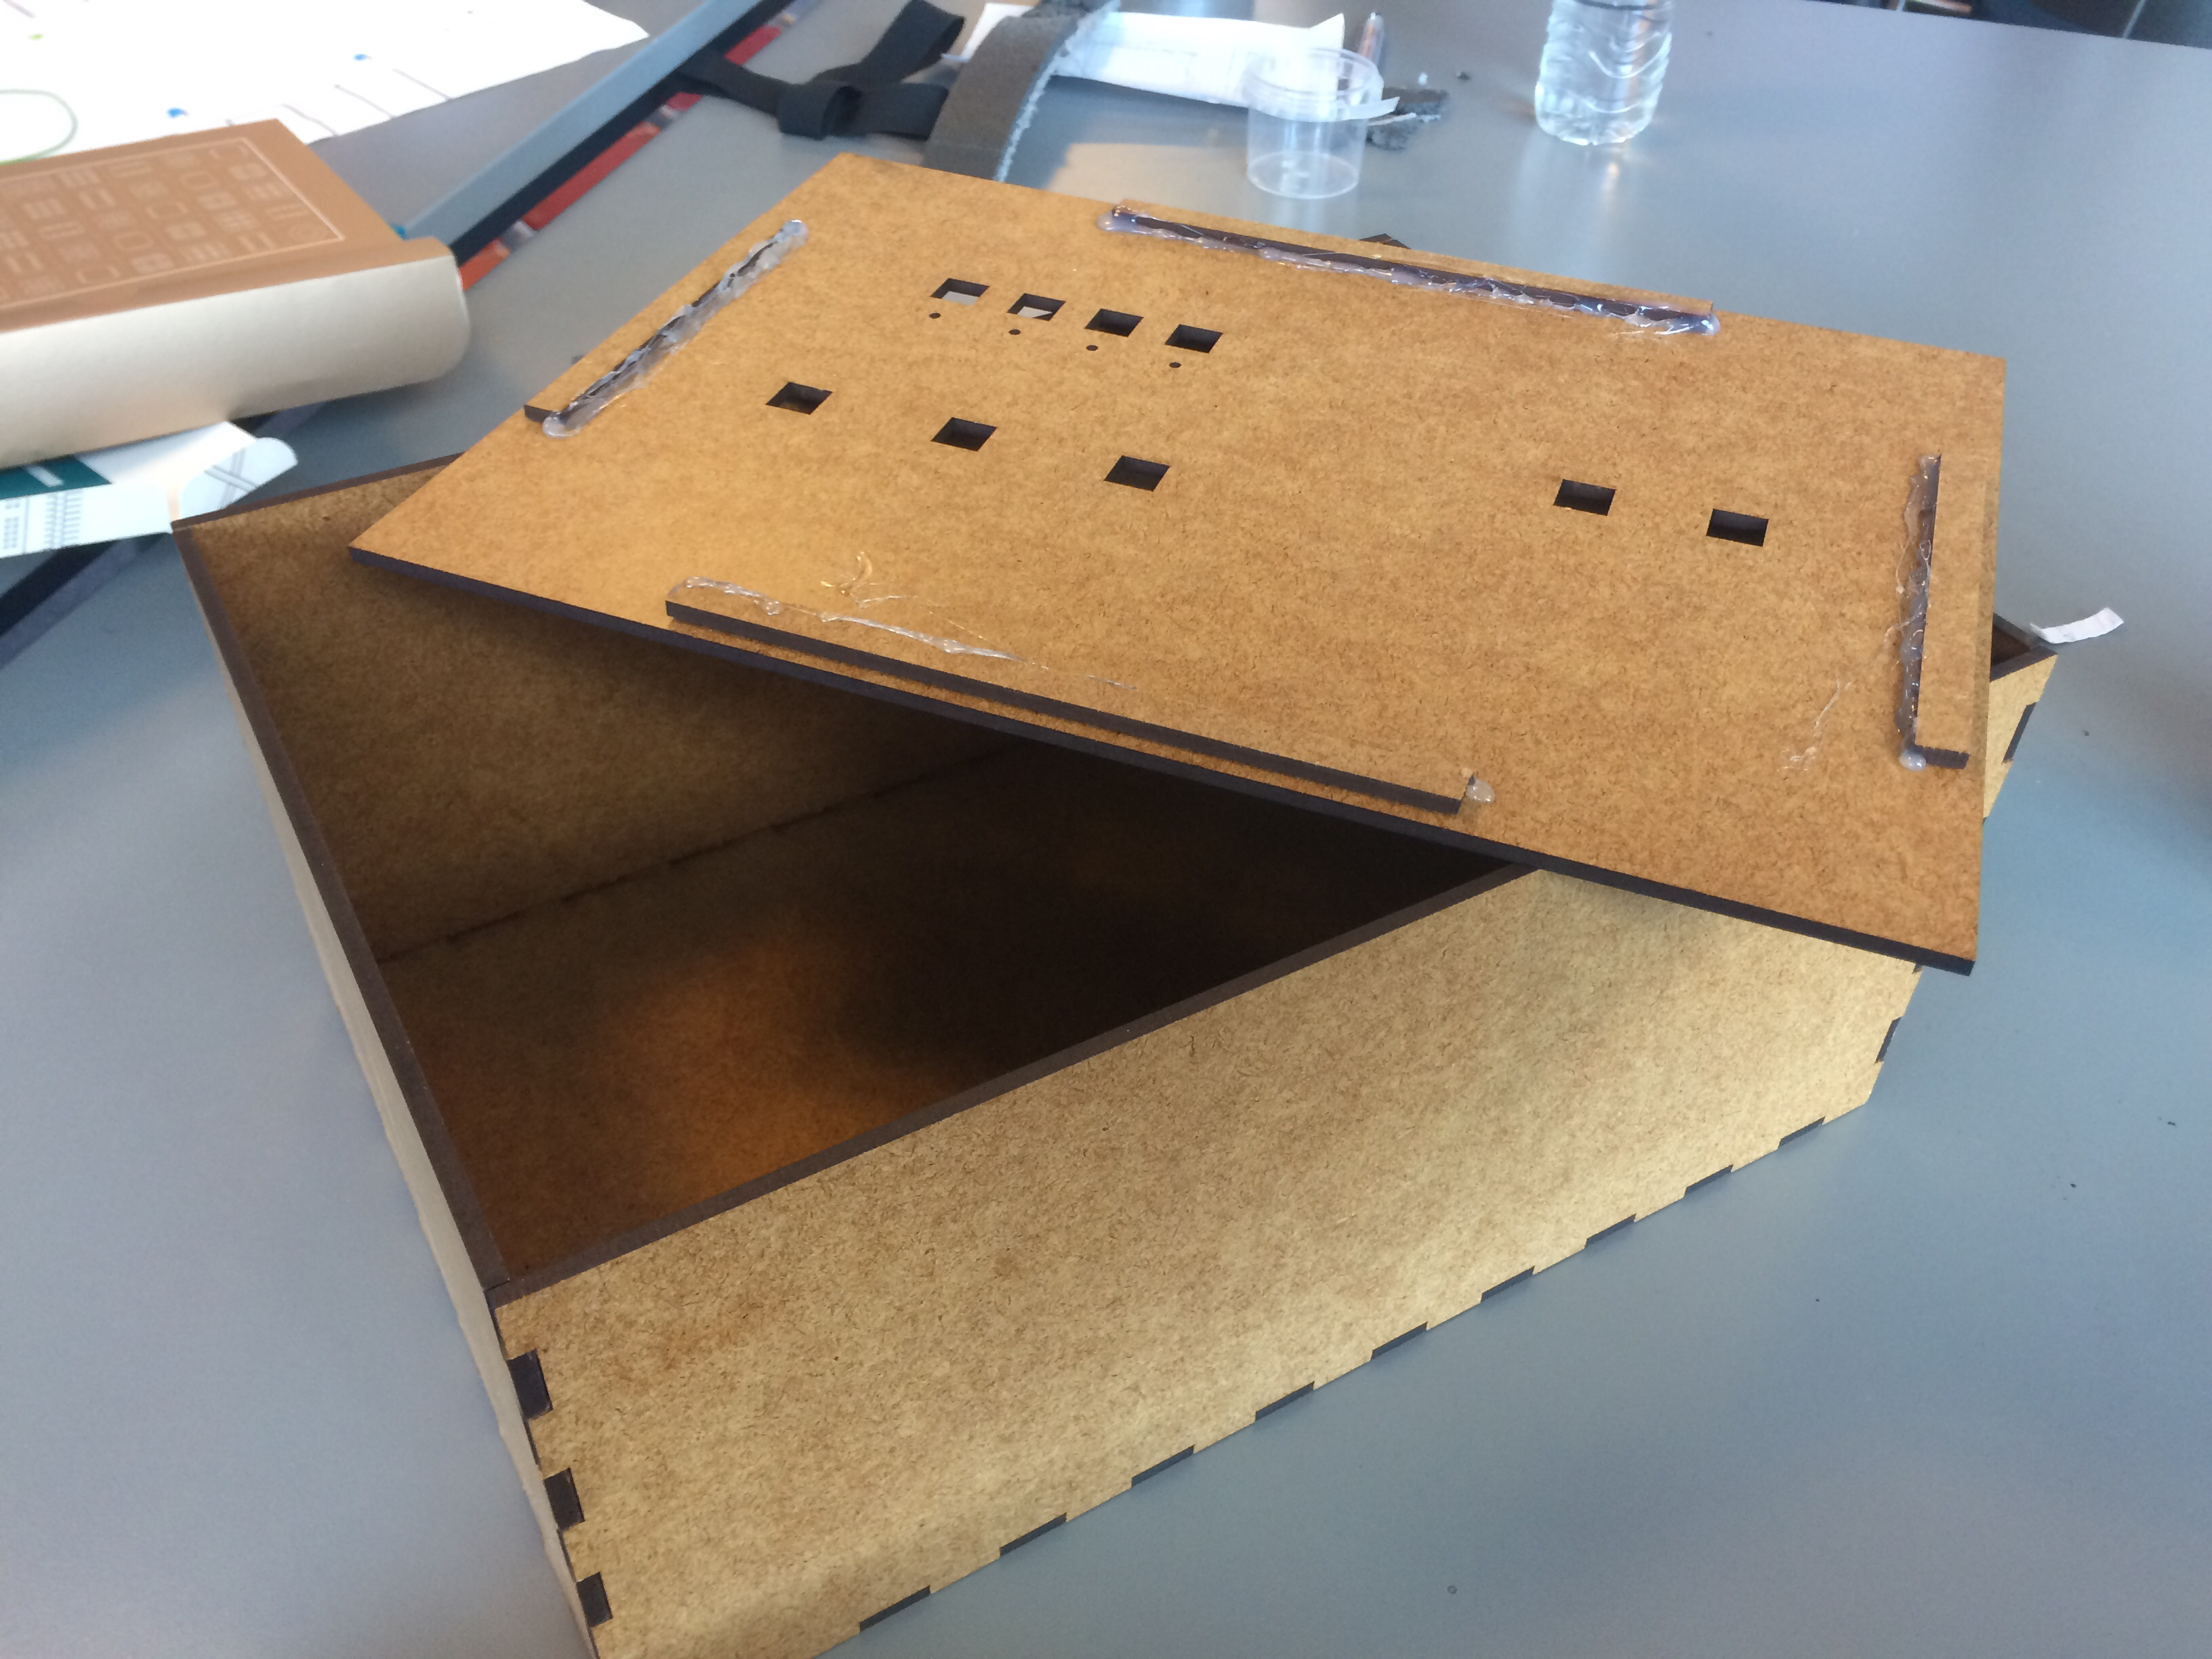
\includegraphics[width=0.7\linewidth]{figure/Design/finalbox2}
	\label{fig:finalbox2}
	\caption{The final prototype box}
	
\end{figure}

\begin{figure}[H]
	\centering
	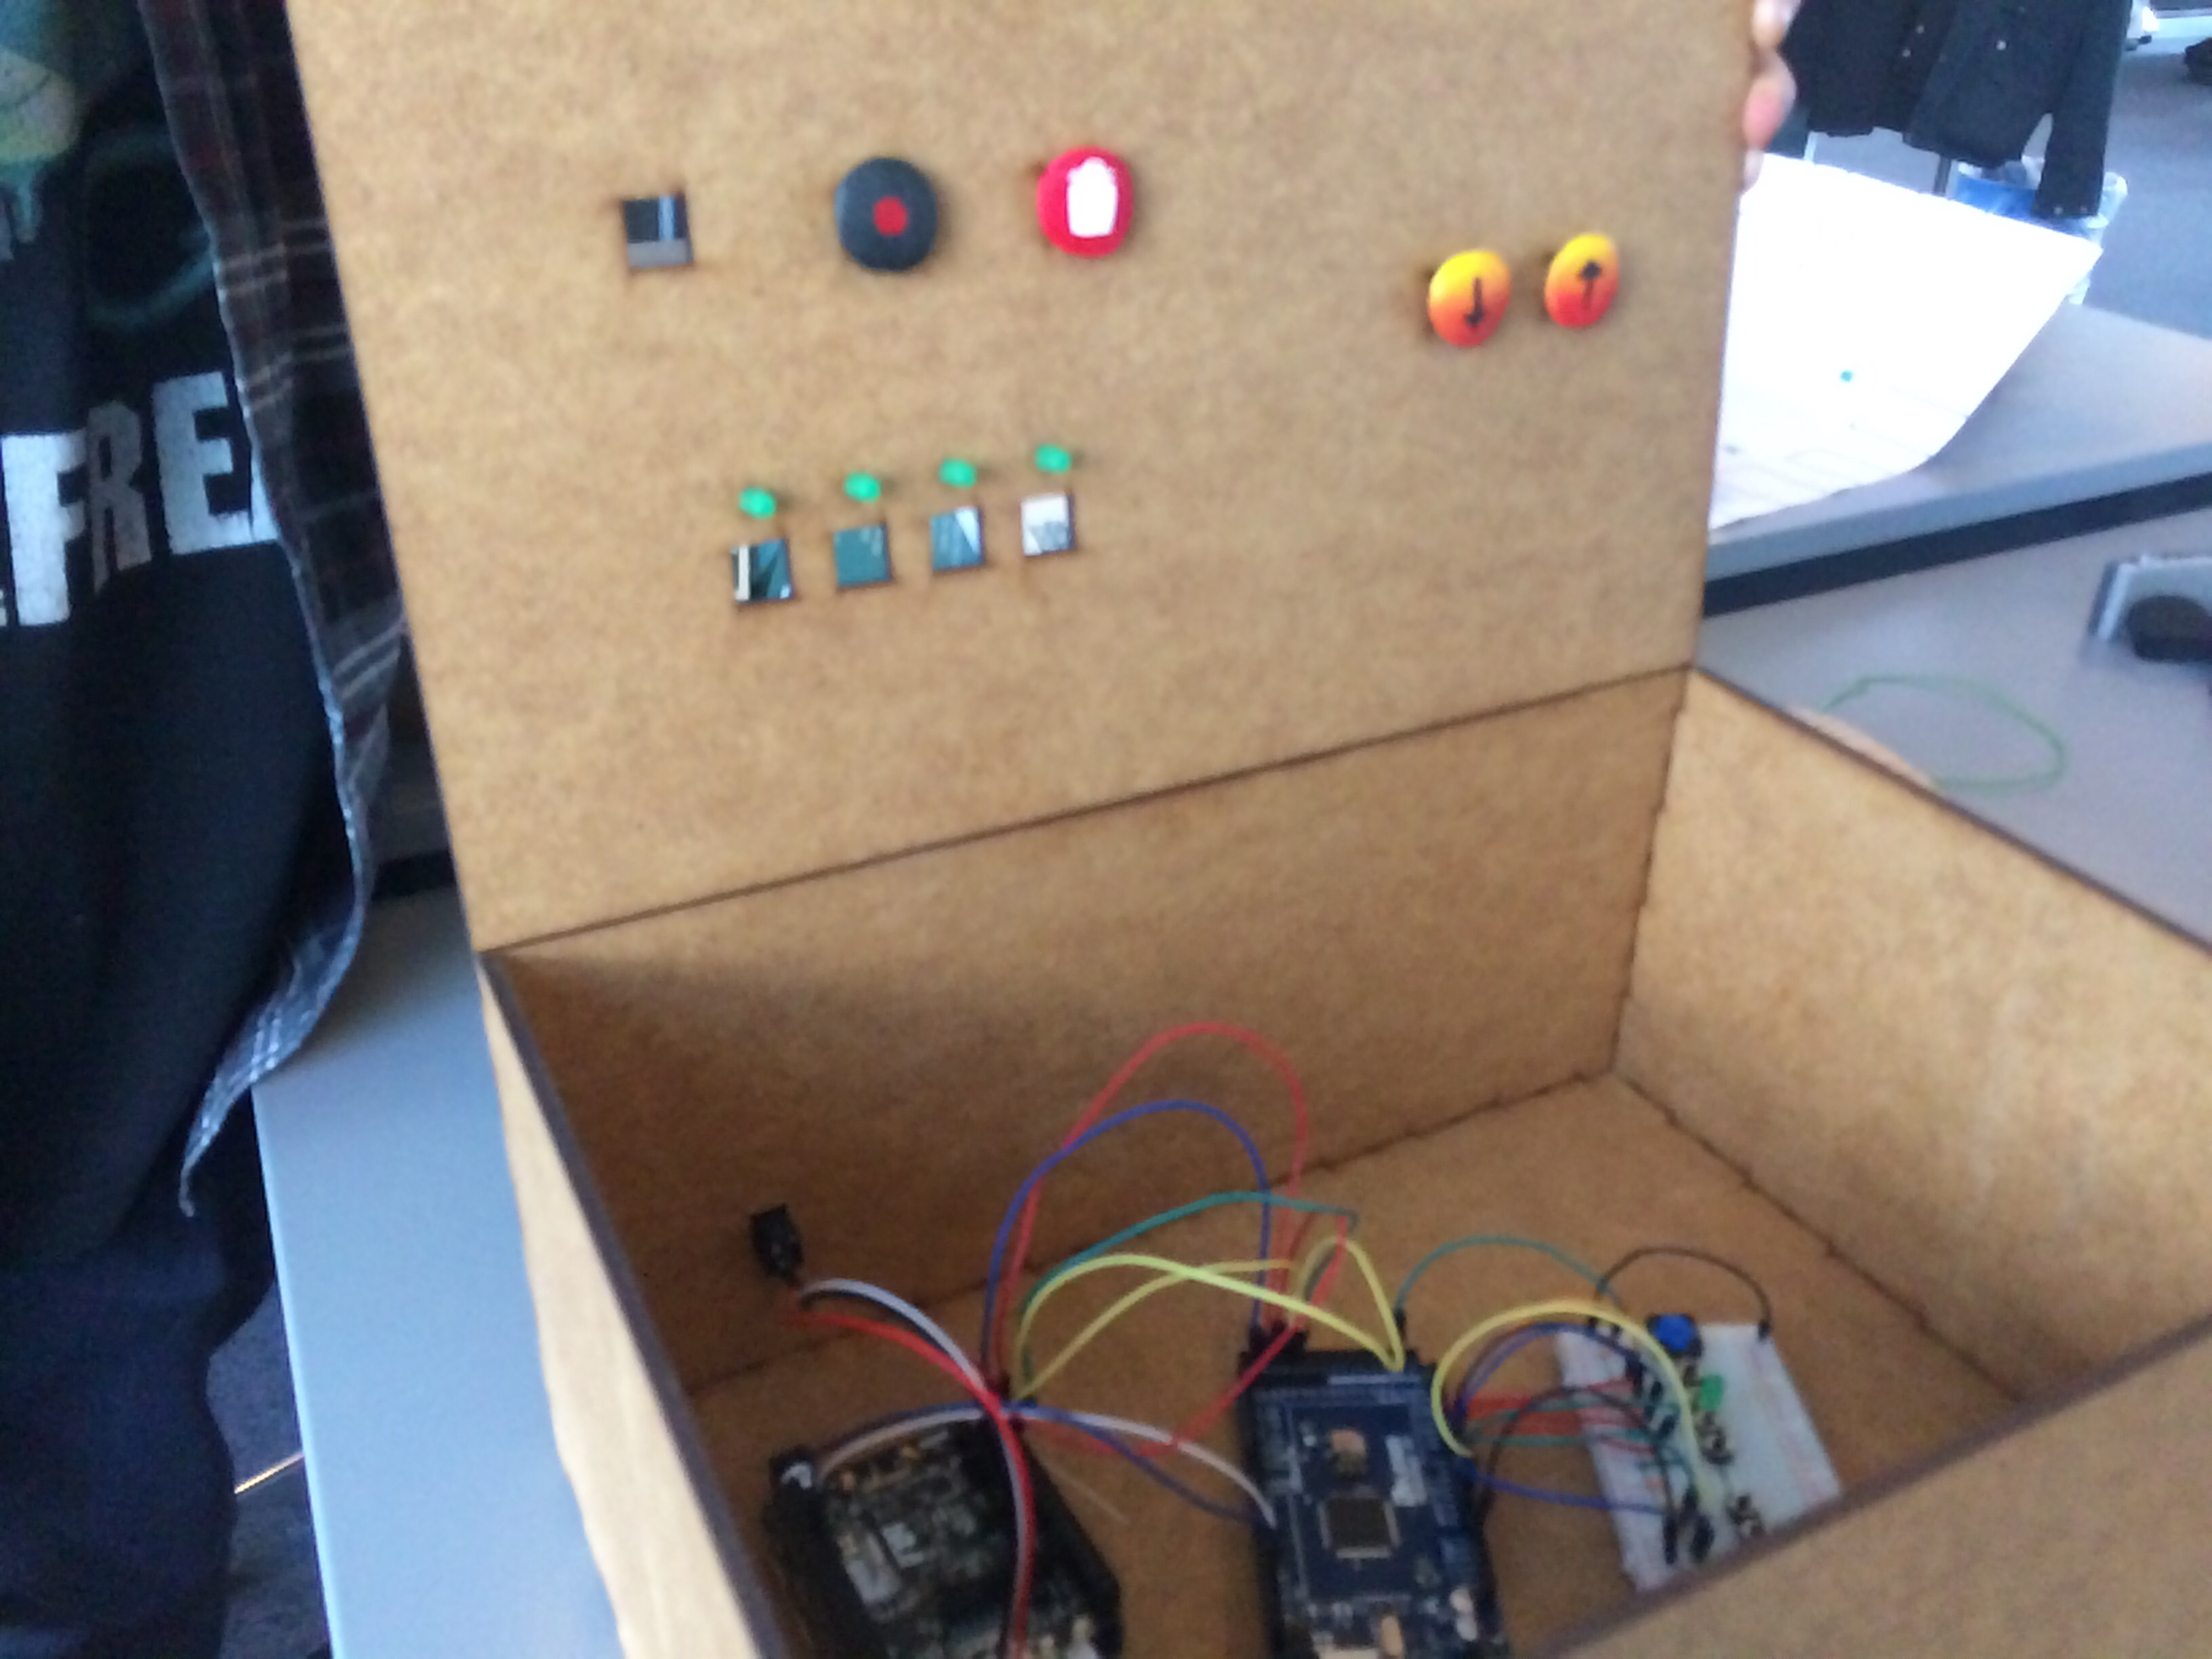
\includegraphics[width=0.7\linewidth]{figure/Design/finalbox3}
	\label{fig:finalbox3}
	\caption{The final prototype box with the eletronic components inside}
	
\end{figure}






